\chapter{Structures discrètes sur l'Internet}

\section{Ressources}
Ressource pour cette partie du cours :\\
Networks, Crowds, and Markets: Reasoning About a Highly Connected World, by David Easley and Jon Kleinberg

\begin{itemize}
\item Chapitre 1-5 (Graphe = modèle des réseaux) définitions, concepts (liens forts et faibles), contexte des réseaux, relations positives et négatives
\item Chapitre 13 (Structure du web)
\item Chapitre 14 (Analyse des liens sur le web)
\item Chapitre 18 (Lois de puissances)
\item Chapitre 20 (Les phénomènes de petit monde)
\end{itemize}

\section{Exemple et analyse de graphes}
Voici quelques commentaires réalisés sur les figures du 1\up{er} chapitre :

\begin{center}
\begin{figure}[!ht]
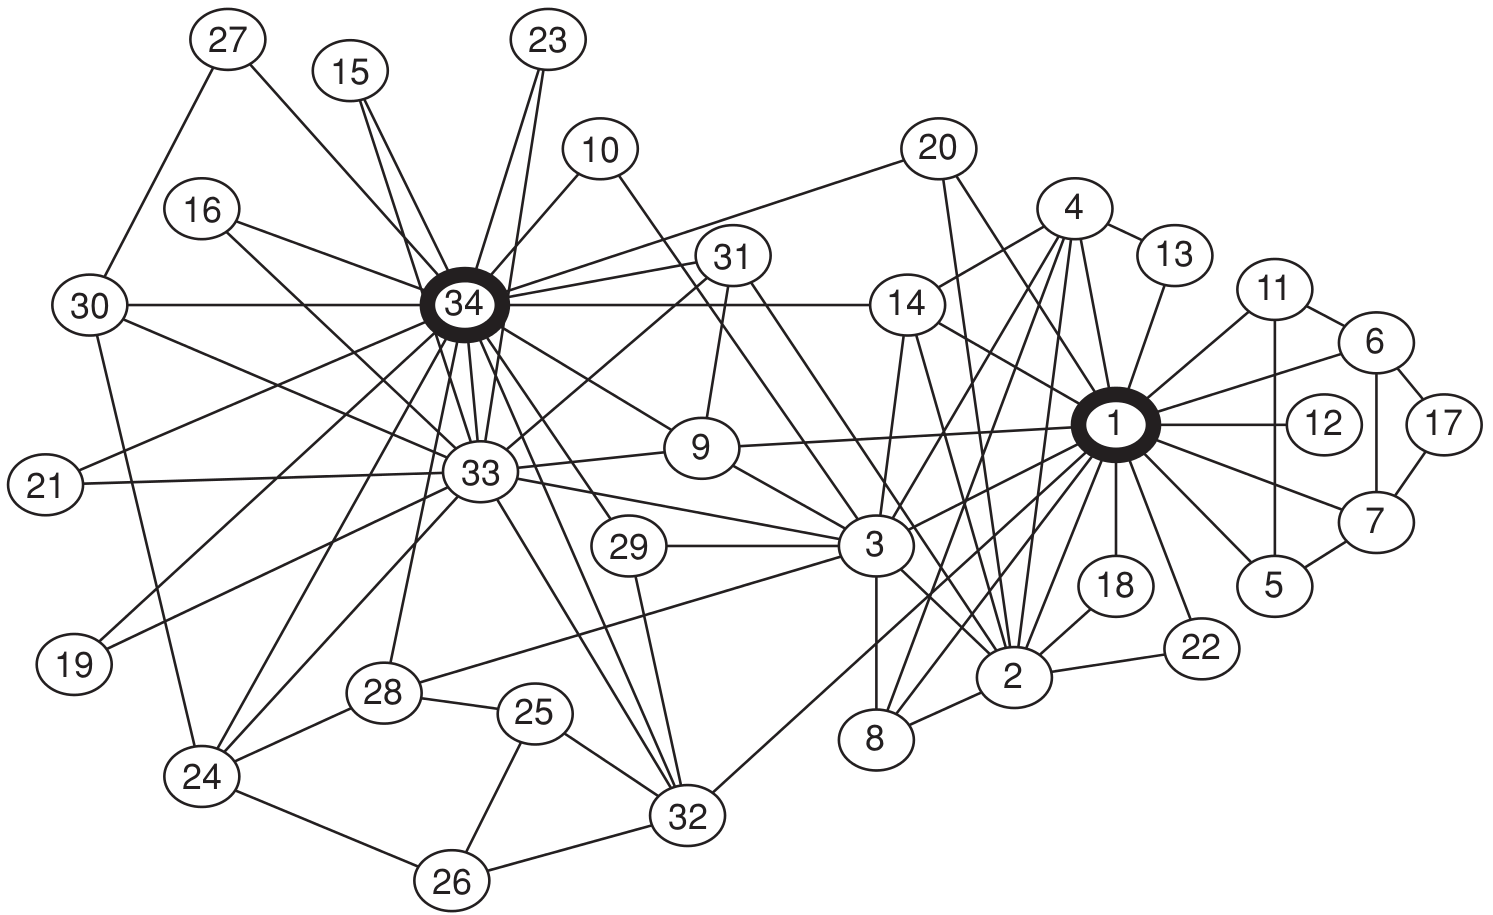
\includegraphics[width=0.75\linewidth]{images/17_karate_club.png}
\caption{Illustration des relations amicales entre 34 personnes dans un
    club de karaté. Chaque n\oe ud représente une personne et chaque lien,
    un lien d'amitié entre ces personnes. On constate que tout le monde
n'est pas ami avec tout le monde. Grâce à cette structure, on peut
déduire certaines choses, par exemple : deux personnes ont beaucoup de
liens d'amitié avec d'autres personnes, mais pas entre eux.}
\end{figure}
\end{center}

\begin{figure}[!ht]
\centering
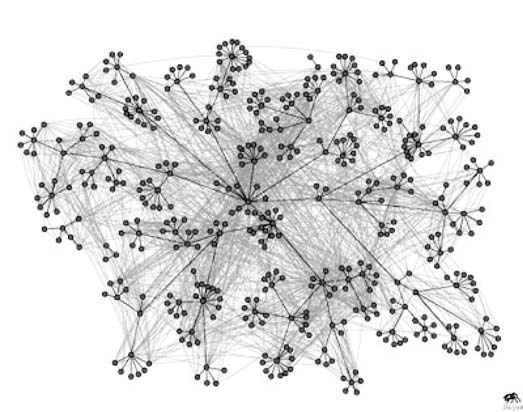
\includegraphics[width=0.75\linewidth]{images/social_networks_based_on_communication_and_interaction.png}
\caption{Des employés dans un laboratoire de recherche (n\oe ud) ont des
    liens entre eux : Lignes claires = communication e-mail. Lignes
    foncées = hiérarchie, organisation du laboratoire. On voit que la
    communication entre les gens suit relativement bien la structure
    hiérarchique, mais pas complètement. On peut voir comment les gens
collaborent, leurs degrés de collaboration, etc.}
\end{figure}

\begin{figure}[!ht]
\centering
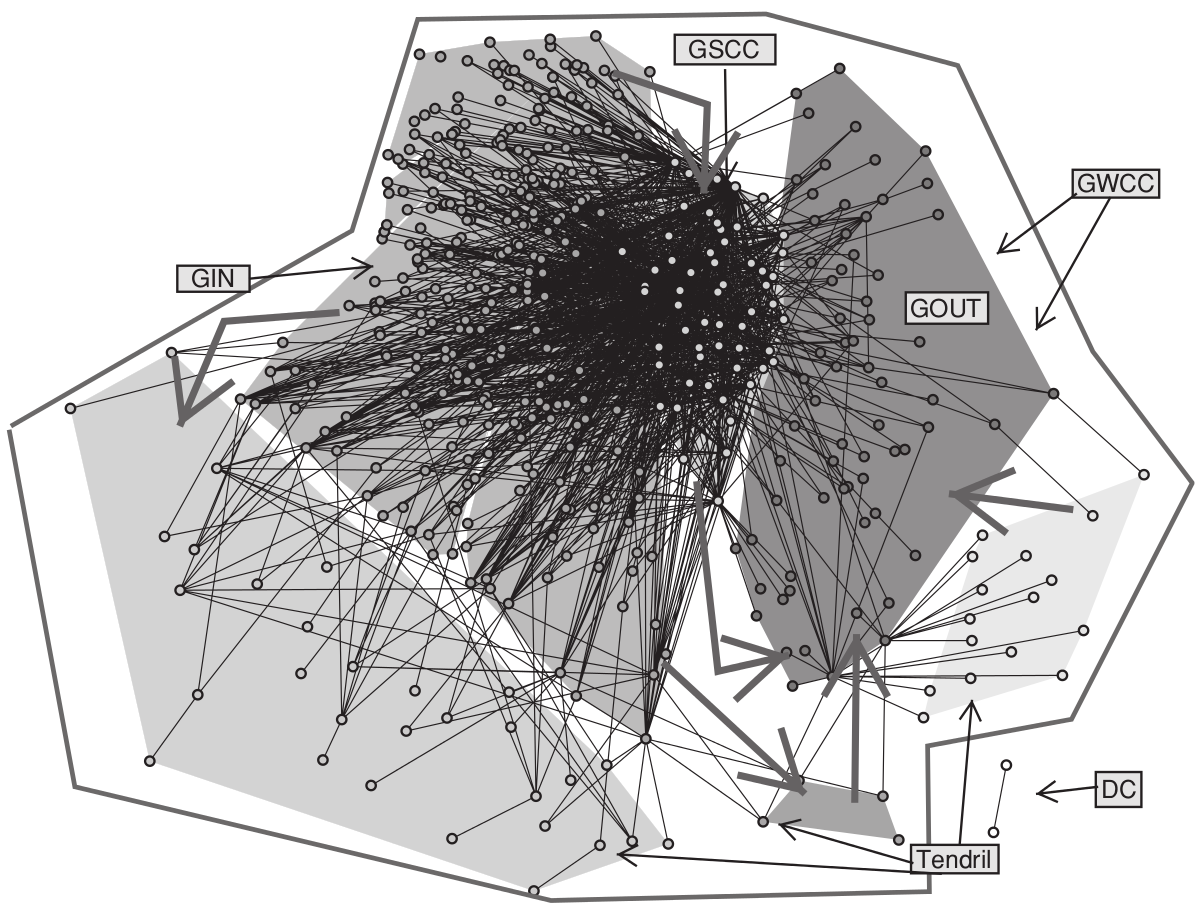
\includegraphics[width=0.65\linewidth]{images/reseaux_prets_entre_banques.png}
\caption{On constate que dans cette illustration, il y a beaucoup plus
    de nœuds. Chaque nœud est une institution financière (banque par
    exemple). Les liens représente des relations entre les banques,
    c'est à dire des prêts faits par une banque à une autre. Le graphe
    est connexe (il y a des chemins entre toutes les banques). Le centre
    est très dense, ça montre une faiblesse du système financier : si
    une banque dans le centre fait faillite par exemple, toutes les
    autres banques liées à elle sont également mises en danger . Donc si
    le noyau central est trop grand, c'est une faiblesse. En regardant
    cette structure, on peut trouver les faiblesses et les comprendre.
Ça peut être très important.}
\end{figure}

\begin{figure}[!ht]
\centering
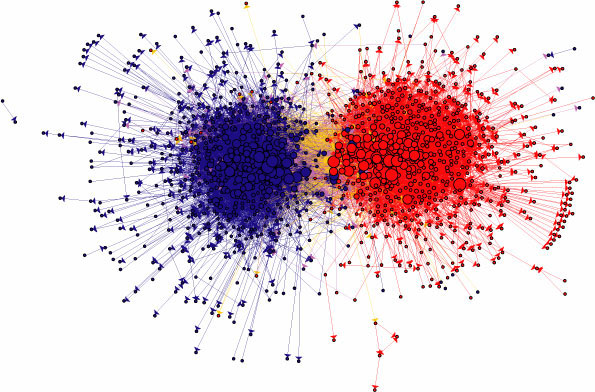
\includegraphics[width=0.65\linewidth]{images/network_structure_of_political_blogs.png}
\caption{Un n\oe ud représente un blog politique et un lien, une référence
    vers un autre blog. Nous avons deux partis qui représentent chacun
    un noyau : les démocrates et les républicains. On constate qu'il y a
    moins de connexions entre les deux noyaux qu'à l'intérieur de
    ceux-ci. On peut visualiser cette structure et se poser des
    questions : est-ce que cette absence de contact entre les deux
factions d'un monde bipolaire est un problème ?}
\end{figure}

\clearpage

Ce sont divers exemples que nous allons essayer d'analyser. Sur Internet, il y a beaucoup de nœuds avec de grandes capacités de calcul et de stockage. Grâce à de nouveaux outils utilisés sur internet pour analyser l'information, on peut observer la structure des graphes (ce qu'on ne pouvait pas faire avant).

\section{Introduction}

Comme montré dans la section précédente, l'analyse des interactions
entre des personnes ou des entités distinctes se fait à l'aide de
graphes. Ces graphes reprennent deux éléments : les entités qui
correspondent à une forme qui peut varier en taille et les liens entre
ces entités qui sont représentés par des lignes. \newline

La structure en réseaux est très présente pour décrire les relations
entre les personnes sur Internet (à travers des réseaux sociaux comme
Facebook et Twitter) et également dans le monde économique (comme
l'exemple des liens du monde bancaire dans la section précedente).
\newline

L'intérêt de la représentation en graphes est de pouvoir montrer les
liens entre des interactions \textit{locales} et leurs conséquences
\textit{globales}. \newline

Il se peut que certaines actions sur les réseaux aient des résultats
contre-intuitifs. Prenons l'exemple d'un réseau routier où il y a des
bouchons, si on augmente la capacité du réseau en ajoutant une voie, les
résultats contre-intuitifs peuvent être multiples :

\begin{enumerate}
    \item Réduction des transferts ;
    \item Augmentation du traffic.
\end{enumerate}

Ce genre de résultats est repris sous l'appellation \textbf{Paradoxe de
Braess}. Concrètement, l'ajout d'une nouvelle capacité sur un réseau
peut réduire la performance globale du réseau (l'explication vient du
fait que chacun tente d'améliorer son temps en trajet personnel en
empruntant la nouvelle route et dans un environnement non-régulé, cette
situation peut déteriorier la performance globale).

\section{Nouvelle discipline}
Les graphes et leurs propriétés évoluent avec le temps, ce n'est pas statique.

Nouvelles disciplines pour analyser des graphes d'informations tirés de sites comme YouTube, Flicker, etc.

Synthèse de 3 disciplines :
\begin{enumerate}

	\item Mathématiques : théorie des graphes
	\item Mathématiques : théorie des jeux\\
		Exemple : YouTube impose ses règles, c'est le croupier, et ceux qui utilisent YouTube sont des joueurs.
	\item Sociologie : étude des groupes sociaux\\
		les participants sont humains ou guidés par un humain. Il n'est pas uniquement question de mathématiques, il faut aussi comprendre les humains.
\end{enumerate}

Dans ce cours, nous nous concentrerons principalement sur la théorie des graphes. La théorie des jeux sera abordée de façon intuitive, et nous parlerons un peu de la sociologie.

\subsection{Théorie des jeux}
On a un ensemble de participants qui jouent à "un jeu" (un ensemble de règles suivies par tous les participants). Chaque participant doit agir : 

\begin{itemize}
\item Simple à spécifier (comme les échecs : 2 participants et 1 action en alternance). 
\item Compliqué : pas d'alternance, tout le monde agit en même temps. C'est un système concurrent.
\end{itemize}

Exemple d'action simple : la vente aux enchères : 
	nombre fini de participants,
	règles simples et définies (différentes techniques sont possibles)
	
\vspace{1cm}

On va rester intuitif sur ce sujet, mais si on veut être plus précis, il y a des champs mathématiques qui étudient les systèmes concurrents.

Enfin, on peut aussi voir que la position dans le graphe peut aussi apporter des avantages.

\begin{figure}[!ht]
\centering
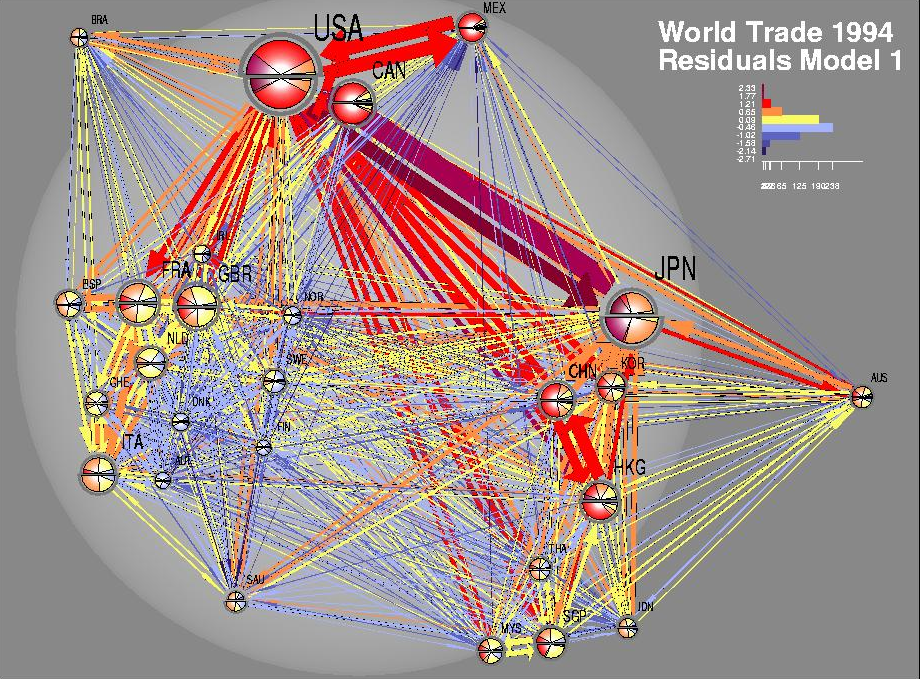
\includegraphics[width=0.8\linewidth]{images/network_international_trade.png}
\caption{Réseau d'interaction économique entre pays. Structure de
    l'économie mondiale : Hong Kong a un gros avantage, il a une porte
    d'entrée vers la Chine (à l'époque). Certains pays sont des
partenaires privilégie des États-Unis...}
\end{figure}

\begin{figure}[!ht]
\centering
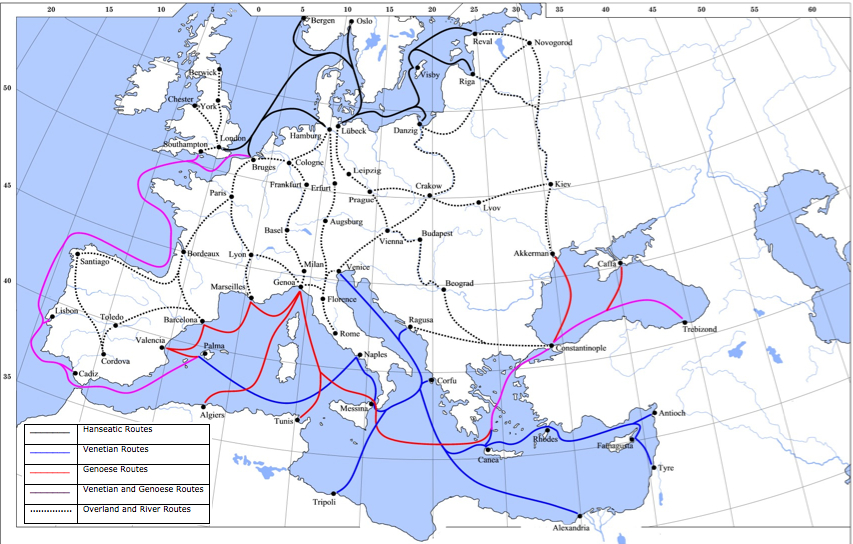
\includegraphics[width=0.9\linewidth]{images/map_of_medieval_trade_routes.png}
\caption{Chemins de commerces médiévaux en Europe. Une position
    stratégique donne des avantages. Tous ces avantages viennent de la
    structure du réseau (notons que le comportement d'un participant
peut dépendre de la structure).}
\end{figure}

Si on observe correctement le réseau, on peut se placer en position d'avantage et se mettre à une position qui donne plus de pouvoir.

Si on connaît la structure, une petite action peut suffire pour arrêter une épidémie en coupant les liens par lesquels cette épidémie pourrait se répandre.
